\chapter{Ergodic Ensemble Approach to the Material Discovery} \label{chap:crystall}

\acknowledge{
This chapter adapts parts of a manuscript draft planned for publication around the dissertation submission, co-authored with Ricardo Amaral, Jonathan W. Siegel, Rushi Gong, ShunLi Shang, and Zi-Kui Liu. All of included text was written by Adam M. Krajewski. Described software has been developed by Adam M. Krajewski since 2020 and by Ricardo Amaral since 2024, with Rushi Gong and ShunLi Shang developing it through testing-feedback loop. ShunLi Shang and Zi-Kui Liu provided edits and guidance. It also adapts excerpt written by Adam M. Krajewski for \citet{Im2022ThermodynamicModeling}. 
}

\section{New Stable Structure Prediction?} \label{crystall:sec:newstable}

The ability to determine atomic structure of existing or hypothetical solids formed by chemical elements is one of the fundamental challanges in theoritical crystallography and in materials science as a whole. For the last several decades \cite{Hawthorne1994}, the two remaining challenges are predictions of (a) compositions forming compounds of interest and (b) candidate topologies or approximate atomic arrangements they can form. Given these, the exact structure can be solved experimentally, by matching X-ray diffraction profile to candidates using the method by \citet{LeBail1988} and interpreting the profile, or using deep learning \cite{Yue2024}. Similar analysis can be done, e.g., on the Raman spectrum \cite{Ferrari2013}. For hypothetical compounds in their pure states, the exact structure can also be solved using ab initio quantum mechanical methods, such as Kohn-Sham density functional theory (DFT) \cite{Kohn1965}, which are computationally expensive but can provide accurate results and continue to improve \cite{Kothakonda2023}.

The latter problem of proposing the topologies has been traditionally approached by finding geometries satisfying constraints, like the principles systematized by [@Pauling1929], which included then-novel concepts like coördination. Over decades, this has evolved into automated computational tools like the \texttt{GRINSP} by \citet{LeBail2005} which can propose such structures. More recently, increasing computational power shifted focus towards testing many options, with some of the methods starting from random arrangements and collapsing them into local minima, like \texttt{AIRSS} by \citet{Pickard2011}, or by evolutionary techniques, like \texttt{USPEX} \cite{Glass2006}. 

Several efforts have been made to tackle both topological and compositional challenges simultaneously, such as high-throughput construction of the \texttt{AFLOW} \cite{Curtarolo2012} DFT Database \cite{Toher2018} (and others, described in Chapter \ref{chap:mpdd}) built by systematically populating the earlier, yet continuously growing, library of prototype structures \cite{Mehl2016} with new chemistries based on the expert knowledge. However, even for a limited set of elements, this problem becomes combinatorically challenging \cite{Krajewski2024Nimplex}. This prompted recent efforts into (1) systematic similarity-driven prediction of substitutions which would result in finding new low-energy structures \cite{Wang2021}; (2) into brute-force substitutions filtered by machine learning (ML) models \cite{Schmidt2023}; and (3) the combination thereof in \citet{Ye2022} and \citet{Merchant2023}, leading to rapid discovery of new structures stable at 0K temperature and 0Pa pressure against competing arrangements.

While finding new candidates for zero-temperature zero-pressure hypothetical structures certainly opens the world for new discoveries, it warrants some key questions. Firstly, *"To what degree have we biased the discovery of new structures?"* through many iterations of biasing the search to our expectations, which is philosophically analogous to how retraining Large Language Models (LLMs) and other ML models on generated data makes them underestimate improbable events causing, so called, *Model Collapse* \cite{Shumailov2023}, and drift from the distribution of the real data \cite{Alemohammad2023}. In the context of materials, the latter is depicted well by Fig. 5 in \citet{Ye2022} showing relatively small overlap between experimentally known structures and new ones predicted to be stable.

In case the data becomes biased towards low-energy solutions, one needs to ask \textit{"Do we need the diverse energy landscapes to discover new materials?"} to which the answer is a multifaceted yes. First, the metastable are critical to fitting thermodynamic models as protodata, as highlighted in study by \citet{Olson2023}, which also stresses that at the same time, computational thermodynamics models \emph{phases} which, at finite temperatures, represent ensembles of underlying configurations and structures. 

Furthermore, one has to consider that going beyond highly-stable materials is needed to create realistic model, as concisely explained by \citet{Zunger2019}, because of the several complexities involved in the synthesis of new materials, such as defect modeling. 

Once such realistic models are obtained, coexistance of many configurations can be used to accurately (1) take properties to extremes, e.g. infinitely negative thermal expansion modeled by \citet{Liu2022} to match the experiments without arbitrary fitting parameters, or (2) model superconductors \cite{Ferreira2023}. Thus, efforts to generate ensembles of possible structure candidates need to propose diverse polymorph populations, such as one in Fig. 6 in \citet{Pickard2011} generateed through \texttt{AIRSS}.


\section{\texttt{crystALL} - Purely Data-Driven Structure Prediction for Unidentified Chemical Compounds} \label{crystall:sec:crystall}

At its core, \texttt{crystALL} leverages large local and remote collections of atomic structures, such as \texttt{MPDD} described in Chapter~\ref{chap:mpdd}, to propose new candidates based on matching stoichiometry, i.e., the anonymized formula, as shown in Figure~\ref{crystall:fig:crystallcompound}, while generating all possible permutations of such substitutions (e.g., 6 for $ABCD_4$ compounds). These candidates are then passed into the \texttt{pySIPFENN} \citet{Krajewski2024EfficientStructures}, featurized using \texttt{KS2022} described in Section~\ref{pysipfenn:ssec:ks2022features}, analyzed for uniqueness, and then passed to next stages of filtering.

\begin{figure}[H]
    \centering
    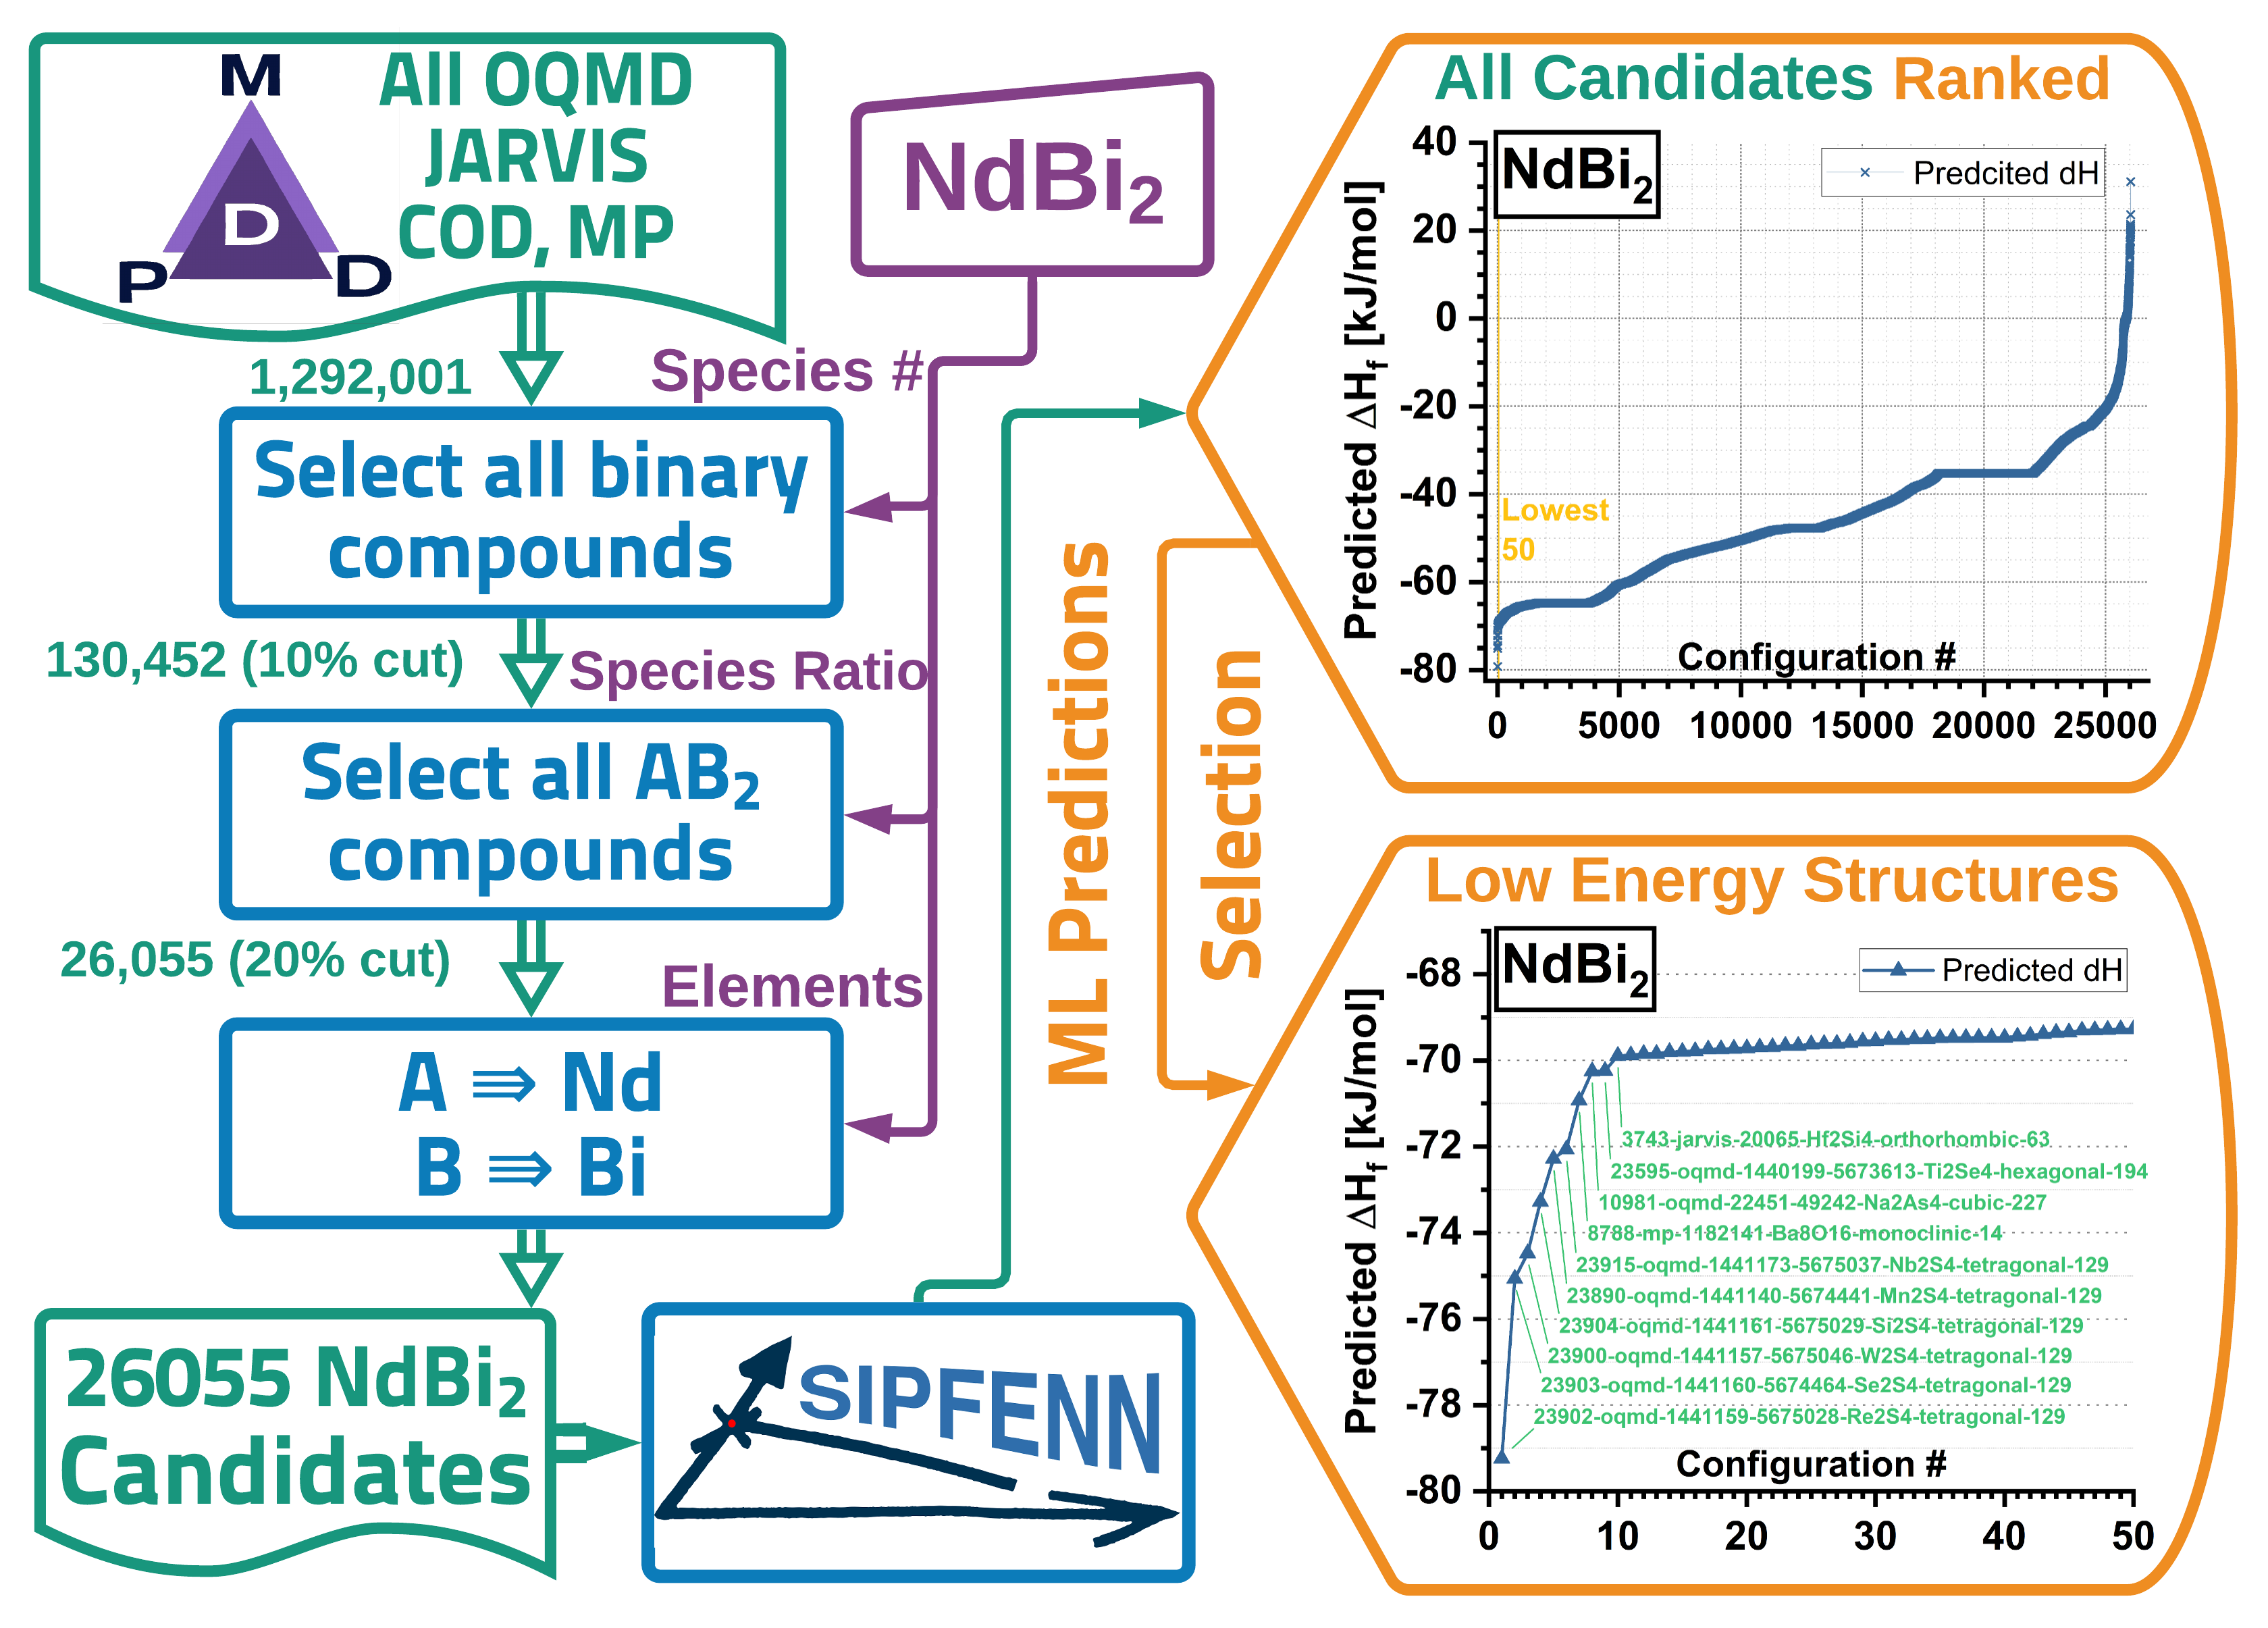
\includegraphics[width=0.75\textwidth]{crystall/NdBi2_GraphicalAbstract_V4.png}
    \caption{Simplified \texttt{crystALL} core schematic of operation based around performing all permutations of elemental substitutions and energy predictions, exemplified in the case of $NdBi_2$ intermetallic.}
    \label{crystall:fig:crystallcompound}
\end{figure}

During the filtering step, selection of candidates is primarily based on the clustering analysis inside the \texttt{KS2022} feature space, with lowest-predicted-energy member of each cluster being selected and \emph{assumed} to be a metastable local minimum of structures belonging to a configuration. Such set of configurations is then passed into DFT-based methods for validation, in the order of predicted stability, until it appears \emph{ergodic} or a structure of interest has been identified. Section~\ref{crystall:ndbi2} discusses all of the above steps on a specific example of \ch{NdBi_2}.


\section{Successfully Identifying \ch{NdBi_2} Structure} \label{crystall:ndbi2}

The first deployment of the \texttt{crystALL} method happened within \citet{Im2022ThermodynamicModeling} work, which re-assessed thermodynamic models of Nd-Bi chemical system, which was an essential step towards the rational design of rare-earth alloys for clean energy technologies through, e.g., electrochemical recovery of rare-earth elements and prospects of novel energy storage devices like liquid metal batteries. As noted in the publication, the \ch{NdBi_2} compound has long been known to be thermodynamically stable \cite{Yoshihara1975Rare-earthBismuthides}; however, its crystal structure has remained unknown, presenting a significant obstacle in using ab initio methods to study it. Using \texttt{crystALL}'s data-mining approach deployed on \texttt{MPDD}, the possible configurations of \ch{NdBi_2} were determined and later validated by DFT-based methods, as depicted earlier in Figure \ref{crystall:fig:crystallcompound}.

First, all of the 26,055 \ch{AB_2}-type configurations were extracted from the contemporary mid-2020 snapshot of \texttt{MPDD}, which at the time had approximately 1.3 million total configurations dataset of DFT-relaxed or experimental structures covering all materials contained in the Open Quantum Materials Database (OQMD), the Materials Project (MP), the Joint Automated Repository for Various Integrated Simulations (JARVIS), and the Crystallography Open Database (COD), described in Chapter \ref{chap:mpdd}. Following the extraction and substitution, all generated candidates have been featurized using \texttt{Ward2017} \cite{Ward2017IncludingTessellations}, and their energies were predicted through \texttt{SIPFENN} Novel Materials Model (NN20) described in Chapter \ref{chap:sipfenn}. The 1,000 lowest energy candidates were selected, and their feature-space representations were embedded into lower dimensional space (3D) using popular t-distributed stochastic neighbor embedding (t-SNE) \cite{HintonStochasticEmbedding} and clustered using k-means approach, as depicted in Figure \ref{crystall:fig:ndbi2clusters}.

\begin{figure}[H]
    \centering
    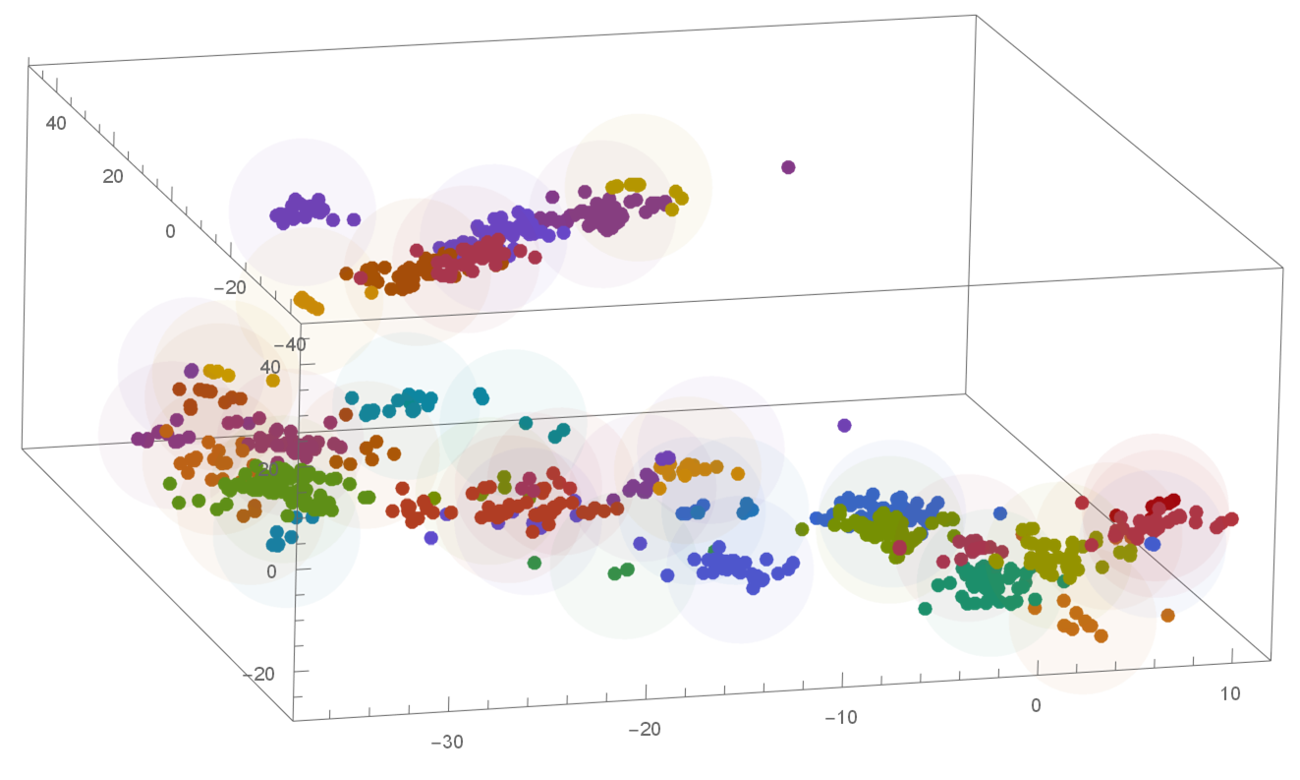
\includegraphics[width=0.8\textwidth]{crystall/crystall_NdBi2.png}
    \caption{\texttt{crystALL}'s t-SNE low-dimensional (3D) embedding of \texttt{Ward2017} feature vectors of 1,000 lowest energy \ch{NdBi_2} candidates, as predicted by \texttt{SIPFENN}, clustered with k-means approach to determine the ensemble of unique structures.}
    \label{crystall:fig:ndbi2clusters}
\end{figure}


Next, the \texttt{SIPFENN}-predicted formation energies were overlaid on the candidate space, as shown in Figure \ref{crystall:fig:ndbi2energies}, and the most stable candidate from each cluster has been selected for further evaluation under 3 different DFT settings in the order of predicted stability.


\begin{figure}[H]
    \centering
    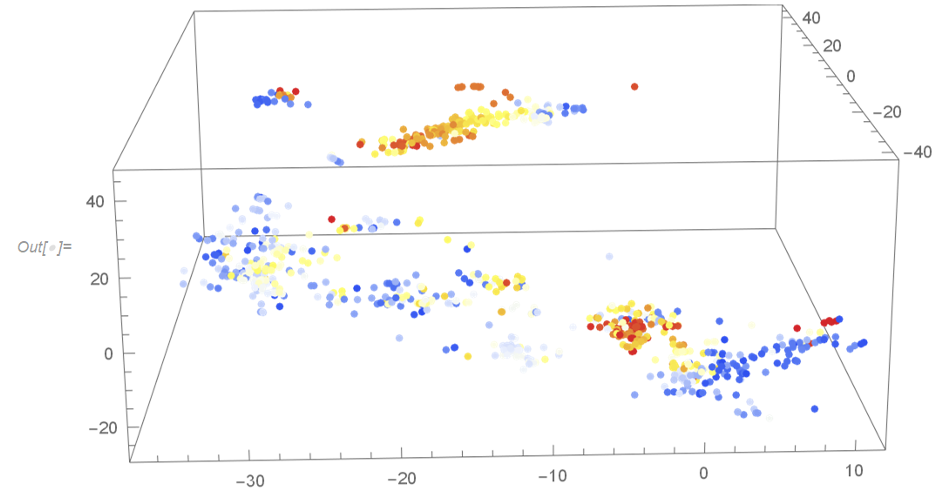
\includegraphics[width=0.8\textwidth]{crystall/crystall_NdBi2_energies.png}
    \caption{\texttt{crystALL}'s t-SNE low-dimensional (3D) embedding of \texttt{Ward2017} feature vectors of 1,000 lowest energy \ch{NdBi_2} candidates overlaid with \texttt{SIPFENN} formation energies depicting low energy ("hot") regions.}
    \label{crystall:fig:ndbi2energies}
\end{figure}


Simultaneously to \texttt{crystALL} method, an alternative, \texttt{USPEX} evolutionary structure search \cite{Lyakhov2013NewUSPEX}, mentioned earlier in Section \ref{crystall:sec:newstable}, has also been deployed and, as shown in Figure \ref{crystall:fig:ndbi2dft}, and found a lower energy structure than any of the 20 generated by \texttt{crystALL}, as shown in Figure \ref{crystall:fig:ndbi2dft}. However, as explained in Section \ref{crystall:sec:newstable}, the 0K lowest energy structure is not necessarily the one being searched for. This has been precisely the case in \citet{Im2022ThermodynamicModeling}, as the XRD patterns have been matched to a mixture of two 0K metastable configurations, denoted by arrows in \ref{crystall:fig:ndbi2dft}, which were present in the \texttt{crystALL}-generated ensemble of states.

\begin{figure}[H]
    \centering
    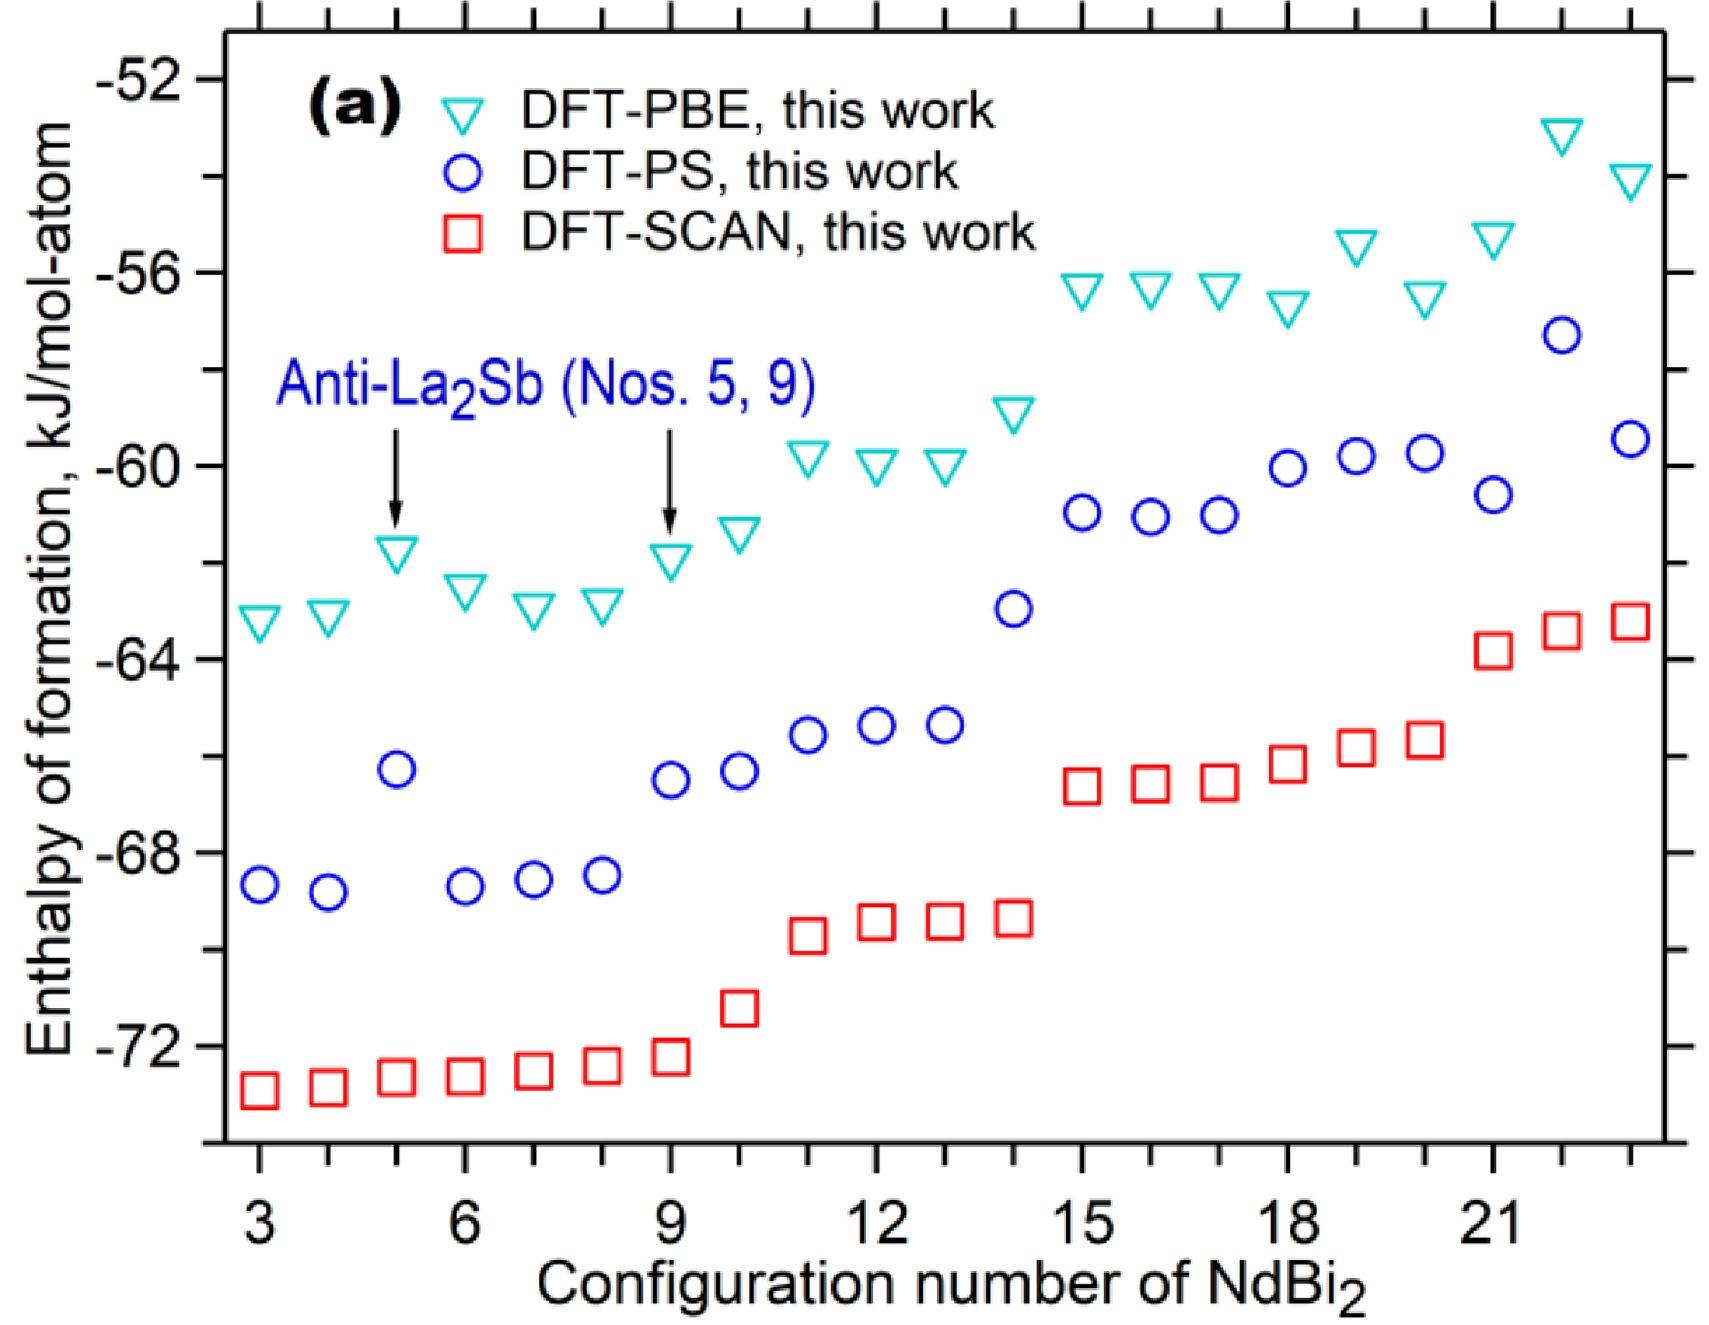
\includegraphics[width=0.6\textwidth]{crystall/crystall_NdBi2dft.jpg}
    \caption{0K formation energies of structure candidates predicted by USPEX (\#3) and \texttt{crystALL} (\#4-23). The mixture of 2nd and 6th lowest-energy candidates has matched the experimental observations of \ch{NdBi_2} demonstrating both \texttt{crystALL}'s predictive ability and criticality of 0K metastable structures.}
    \label{crystall:fig:ndbi2dft}
\end{figure}


\section{Predicting Compounds of Uncertain Compositions} \label{sec:crystallcompositional}

Compound-based searches, discussed in Section~\ref{crystall:sec:crystall} and exemplified in Section~\ref{crystall:ndbi2}, operate based on anonymous chemical formulas which are commonly used for such purpose, either based on expert knowledge \cite{Mehl2016ThePrototypes} or through screenings \cite{Curtarolo2013AFLOW:Discovery, Schmidt2023, Ye2022NovelAgents}, and can be accessed from nearly any atomistic database thanks to \texttt{OPTIMADE} API \citet{Evans2024DevelopmentsExchange}. While powerful, they suffer from a major drawback when used for structure predictions, i.e., they require researcher to specify exact composition of a compound, while the experimental observations can often match many stoichiometries.

Thus, to address this need, \texttt{MPDD} has been extended with a new \texttt{sortedFractionsDict} field holding an ordered list of anonymized and quantized ($0.1\%$) atomic fractions, with associated \texttt{MongoDB} indexing. This enables \texttt{crystALL} to rapidly query for candidate structures falling within a certain range, which can be set accounting for experimentally observed deviations in the measurement, as shown in Figure~\ref{fig:crystallcomposition}.

\begin{figure}[h]
    \centering
    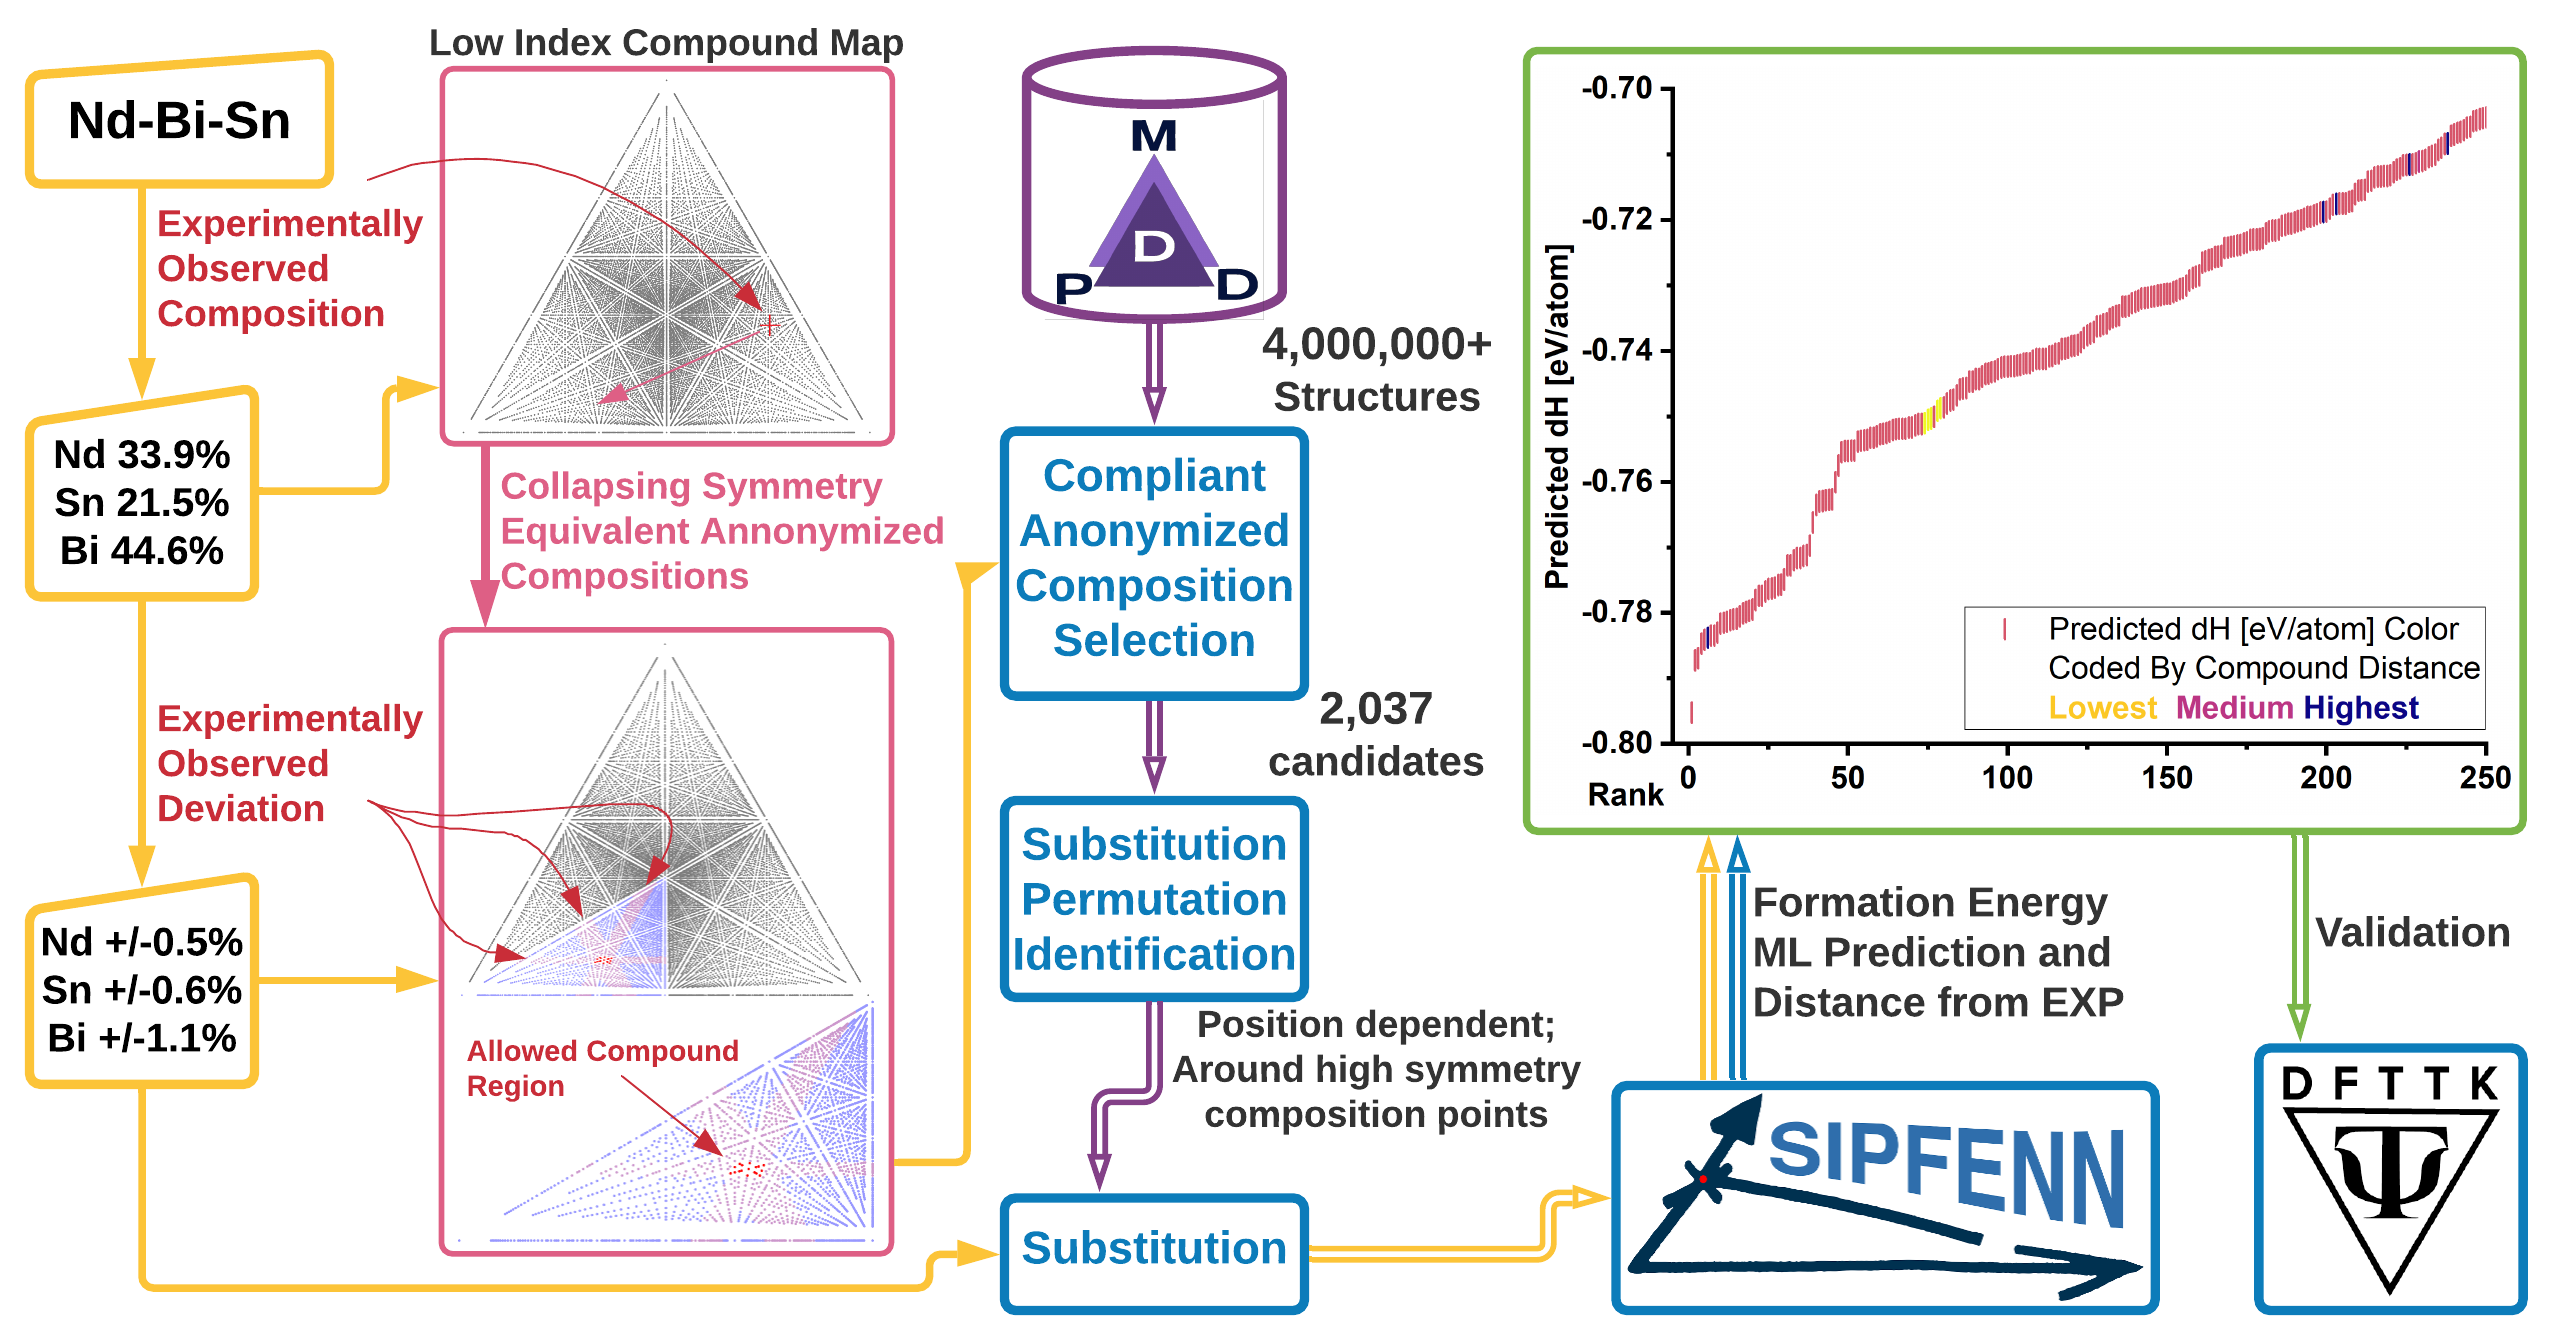
\includegraphics[width=0.95\textwidth]{crystall/crystALL_composition_diagram_V3.png}
    \caption{\texttt{crystALL} schematic of operation in cases of "compositional" searches where measured composition can be given alongside uncertainty bounds. Efficient handling of such queries is a unique feature of MPDD.}
    \label{fig:crystallcomposition}
\end{figure}

Such approach generates output with additional information of the compositional distance to the \textit{reported} composition value, enabling researchers to make a better-informed decision on what to pass into the validation steps based on belief whether the hypothetical compound is the one being observed.

\section{Software Availability} \label{crystall:sec:softwareavaialbility}

The \texttt{crystALL} source code is currently developed closed-sourced; however, it is planned to be released as a free open-source software (FOSS) in the Fall of 2024 through outlets including GitHub repository at \href{https://github.com/PhasesResearchLab/crystALL}{github.com/PhasesResearchLab/crystALL}, alongside a scientific publication describing it, high-quality documentation, and a workshop-style tutorial.

% \section{Connection to Zentropy} \label{sec:crystallzentropy}
% 
% \begin{itemize}
%     \item 
%     \item
%     \item
% \end{itemize}

%\printbibliography[heading=subbibintoc]